\index{color page}

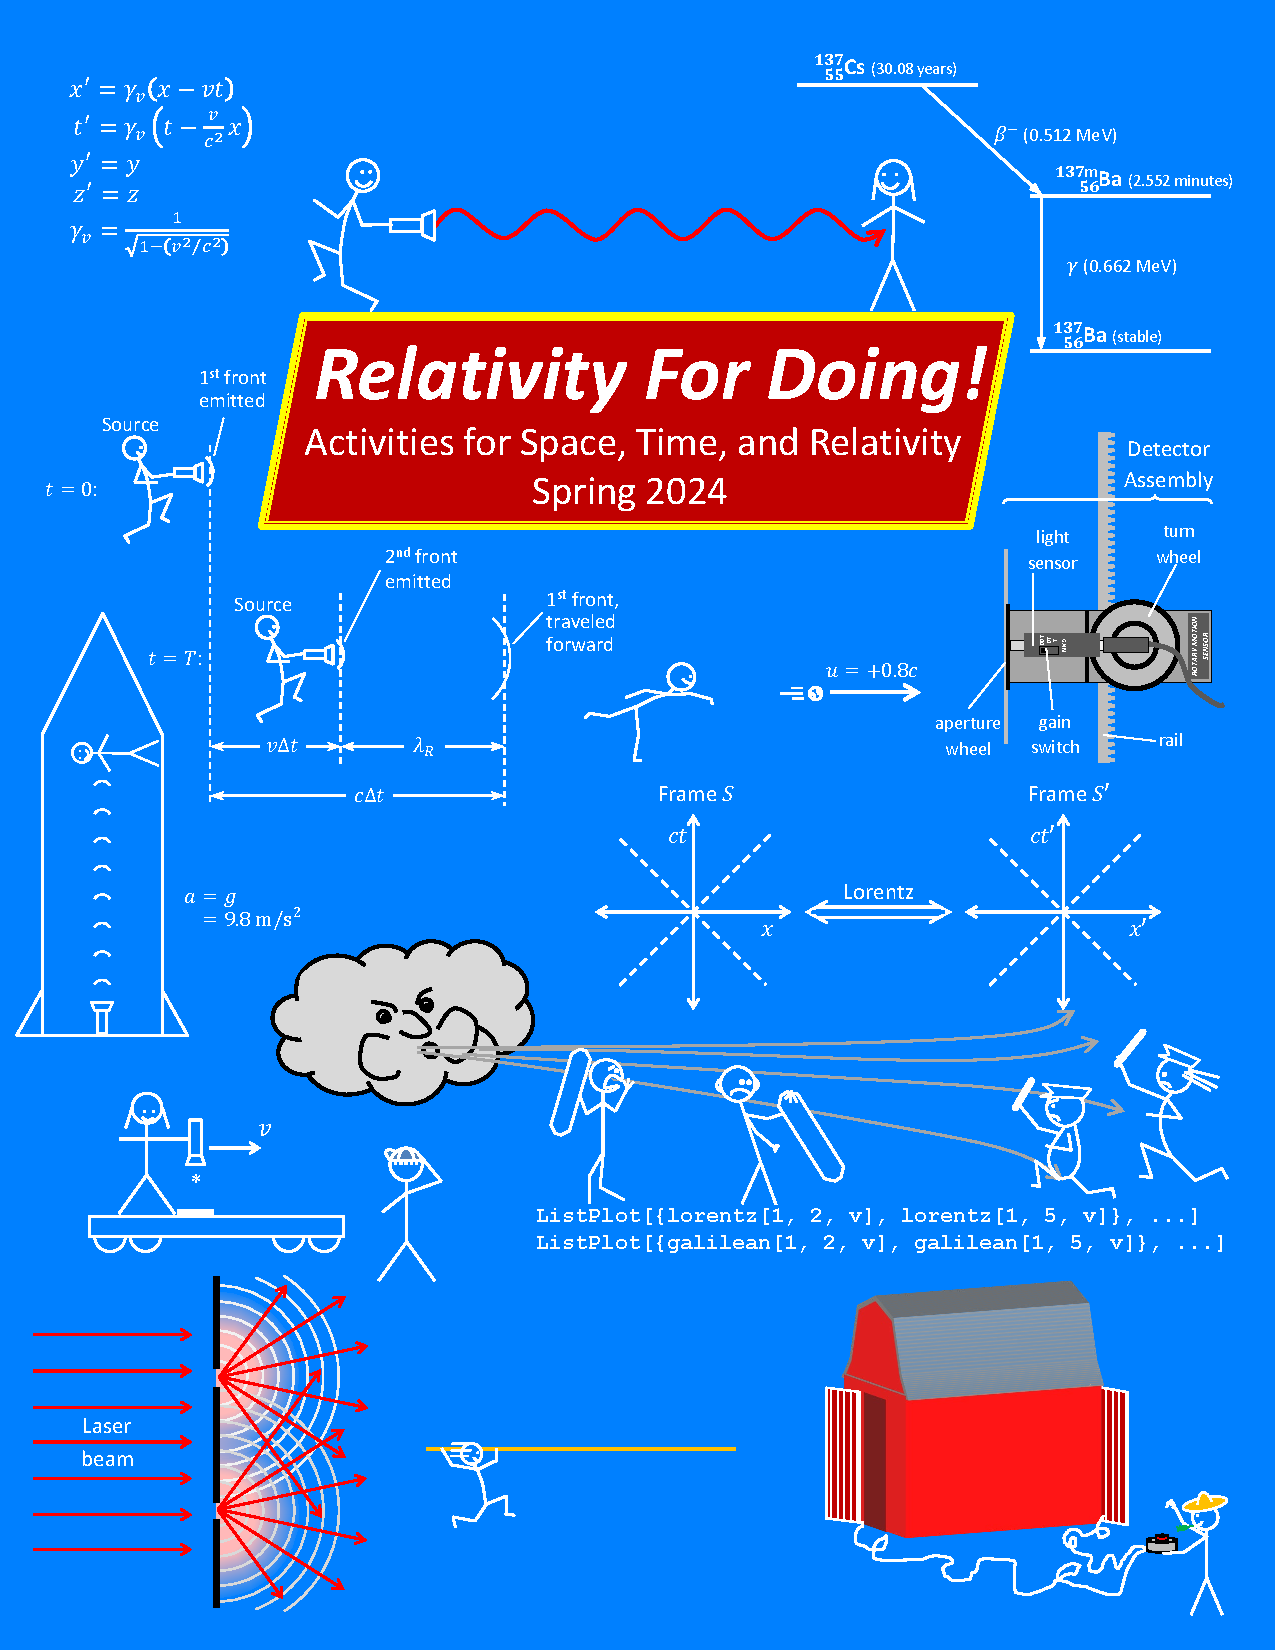
\includepdf[pages=1]{FYS_front_pages/FYS_front_cover.pdf}

\thispagestyle{empty}

\

\vfill
\textit{Cover art: Various graphics and diagrams from the activities in this manual.  You'll be doing lots of stuff.}
\pagebreak



\title{Relativity For Doing!\\
Activities for First-Year Seminar: Space, Time, and Relativity}

%\author{Gerard P. Gilfoyle}
%\author{Jack Singal}
% MT sez: I think I wrote all of the relativity labs that we're going to do here... 
% Jerry wrote the original Nuclear Physics lab.
% From the other lab manuals, I think I'll only use the Doppler effect lab and the two-slit interference lab,
% which I also wrote the current version of.  Happy to add another author if I'm missing anything...
\author{Matthew L. Trawick}
\affil{Department of Physics, University of Richmond, VA}

\maketitle

\vspace{0.8 in}

%\begin{abstract}

\begin{center}
\large{\textbf{Welcome to Space, Time, and Relativity!}}
\end{center}


This manual is a set of exercises for use in the First-Year Seminar section ``Space, Time, and Relativity'' at the University of Richmond, covering various topics in special and general relativity.  These exercises are primarily intended as in-class activities, or ``labs,'' though most of them are kind of fake labs in that they don't use any physical equipment beyond a computer and some software, at most.

MT gratefully acknowledges the advice and assistance of Ted Bunn, both for fielding specific Mathematica questions and for many helpful discussions about teaching this course.

%\end{abstract}


\newpage
\
\thispagestyle{plain}

\newpage
\
